
To test algorithms (\ref{alg:EM-SO}) and (\ref{alg:P-EM-SO}), we ran a total of eight experiments, each of which involved five data sets and five random parameter initializations. For each data set, we simulated a total of $T \in \{10^3,10^5\}$ observations from an HMM with $N \in \{3,6\}$ hidden states and observations $y_t \in \bbR^d$, with $d \in \{3,6\}$. For every experiment and data set, $Y_t | X_t = i$ follows a normal distribution with mean $\mu^{(i)}$, and covariance matrix $\Sigma^{(i)}$. We randomly define $\mu^{(i)}$ and covariance matrix $\Sigma^{(i)}$ for every data set:
%
\begin{equation*}
    \mu^{(i)} \sim \calN(0,I), \quad \Sigma^{(i)} = \text{diag}(e^{-2}), \qquad i \in \{1,\ldots,N\}.
\end{equation*}
%
Note that $\calN(\mu,\Sigma)$ represents a normal distribution with mean $\mu$ and covariance $\Sigma$, and $I$ is the identity matrix.
%
The transition probability matrices depended upon both $T$ and $N$. Denote the true transition probability matrix from a given experiments with $T$ observations and $N$ hidden states as $\Gamma_{T,N}$. For our experiments, we set
%
\begin{gather*}
    \Gamma_{10^3,3} = 
    \begin{pmatrix} 
        0.9 & 0.05 & 0.05 \\
        0.05 & 0.9 & 0.05 \\
        0.05 & 0.05 & 0.9
    \end{pmatrix},
    \qquad
    \Gamma_{10^5,3} = 
    \begin{pmatrix} 
        0.999 & 0.005 & 0.005 \\
        0.005 & 0.999 & 0.005 \\
        0.005 & 0.005 & 0.999
    \end{pmatrix}
    \\
    \Gamma_{10^3,6} = 
    \begin{pmatrix} 
        0.9  & 0.02 & 0.02 & 0.02 & 0.02 & 0.02 \\
        0.02 & 0.9  & 0.02 & 0.02 & 0.02 & 0.02 \\
        0.02 & 0.02 & 0.9  & 0.02 & 0.02 & 0.02 \\
        0.02 & 0.02 & 0.02 & 0.9  & 0.02 & 0.02 \\
        0.02 & 0.02 & 0.02 & 0.02 & 0.9  & 0.02 \\
        0.02 & 0.02 & 0.02 & 0.02 & 0.02 & 0.9  \\
    \end{pmatrix},
    \qquad
    \Gamma_{10^5,6} = 
    \begin{pmatrix} 
        0.999  & 0.0002 & 0.0002 & 0.0002 & 0.0002 & 0.0002 \\
        0.0002 & 0.999  & 0.0002 & 0.0002 & 0.0002 & 0.0002 \\
        0.0002 & 0.0002 & 0.999  & 0.0002 & 0.0002 & 0.0002 \\
        0.0002 & 0.0002 & 0.0002 & 0.999  & 0.0002 & 0.0002 \\
        0.0002 & 0.0002 & 0.0002 & 0.0002 & 0.999  & 0.0002 \\
        0.0002 & 0.0002 & 0.0002 & 0.0002 & 0.0002 & 0.999  \\
    \end{pmatrix}.
\end{gather*}
%
We set the initial distribution to be $\delta \sim \text{dir}(\onevec_N)$ for every experiment and data set.

Let $\bar y$ and $\bfQ$ denote the sample mean and sample covariance of $\{y_t\}_{t=1}^T$, respectively. For inference, we initialized $\theta_0$ as
%
\begin{equation*}
    \mu^{(i)}_0 \sim \calN(\bar y, \text{diag}(\bfQ)), \quad \Sigma^{(i)}_0 = \text{diag}(\bfQ), \qquad i \in \{1,\ldots,N\}
\end{equation*}
%
Throughout the optimization procedure, we assume that $\Sigma^{(i)}$ is diagonal for all $i \in \{1,\ldots,N\}$. Further, we parameterize each diagonal element of the covariance matrix with its logarithm, so we perform inference directly on $\log\left(\Sigma^{(i)}\right)$, where $\log$ is an element-wise operation.
%
We initialized $\eta_0$ as
%
\begin{align*}
    \eta^{(i)}_0 &\sim \calN(0,1), & i & = 2,\ldots,N \\
    %
    \eta^{(i,j)}_0 &\sim \calN(-2,2^2), & i,j & = 1,\ldots,N, \qquad i \neq j.
\end{align*}
%
%If the 2-norm of the average estimated gradient $||\frac{1}{T}\sum_{t=1}^T \widehat \nabla F^{(k,m)}_t + \widehat \nabla G^{(k,m)}_t||$ ever fell below a tolerance of $10^{-8}$, we terminated the M-step of algorithm and moved on to the E-step. Likewise, if the relative change of the log-likelihood after one full E- and M- step of the EM algorithm ever fell below a tolerance of $10^{-10}$, we terminated the algorithm altogether. We found the ground truth MLEs by running the traditional EM algorithm until the relative change in the log-likelihood was on the order of machine precision $10^{-15}$.

We estimated the parameters of the generating model for all five data sets and all 8 experiments using 6 different inference algorithms:
%
\begin{enumerate}
    \item Algorithm (\ref{alg:EM-SO}) with $M=T$, using SVRG
    \item Algorithm (\ref{alg:EM-SO}) with $M=T$, using SAGA
    \item Algorithm (\ref{alg:P-EM-SO}) with $M=T$, using SVRG
    \item Algorithm (\ref{alg:P-EM-SO}) with $M=T$, using SAGA
    \item Algorithm (\ref{alg:P-EM-SO}) with $M=10T$, using SVRG
    \item Algorithm (\ref{alg:P-EM-SO}) with $M=10T$, using SAGA
\end{enumerate}
%
All six algorithms used initial step sizes of $\lambda_F = 1/3 \hat L_F$ and $\lambda_G = 1/3 \hat L_G$. The Lipschitz constants were initialized as $\hat L_F = = \hat L_G = 100/3$ and updated during the optimization routine according to the procedure from section \ref{subsec:est_L}. 

We also estimated the HMM parameters using 3 baseline methods:
%
\begin{enumerate}
    \item BFGS \citep{Fletcher:2000}
    \item Conjugate gradients \citep{Fletcher:1964}
    \item Gradient descent
\end{enumerate}
%
All baselines were implemented using the Python library in Scipy \citep{Virtanen:2019}.
%
All algorithms were run for a total of 12 hours on the Compute Canada Cedar cluster on nodes with 16GB of RAM.
%
Figure (\ref{fig:ll_trace_sim}) displays the log-likelihood (divided by $T$) of the maximum log-likelihood minus the log-likelihood (divided by $T$) at each epoch after 12 hours or 150 epochs (whichever came first) for the first data set and a selected random initialization. For each optimization algorithm we select the random initialization that resulted in the highest likelihood after 12 hours. The dots on each figure correspond to the epoch and likelihood at convergence for each algorithm. Note that our stochastic optimization methods are less prone to getting stuck in local minima, especially when $N=6$. The stochastic optimization methods outperform the baseline methods for all experiments with the exception of $N = 3$ and $d = 3$, where BFGS achieves a higher log-likelihood after approximately 120 epochs. However, BFGS is expected to outperform our first-order methods on a per-epoch basis when very close to the true solution. We recreate Figure (\ref{fig:ll_trace_sim}) for the other four data sets in the supplement.
%
\begin{figure}
    \centering
    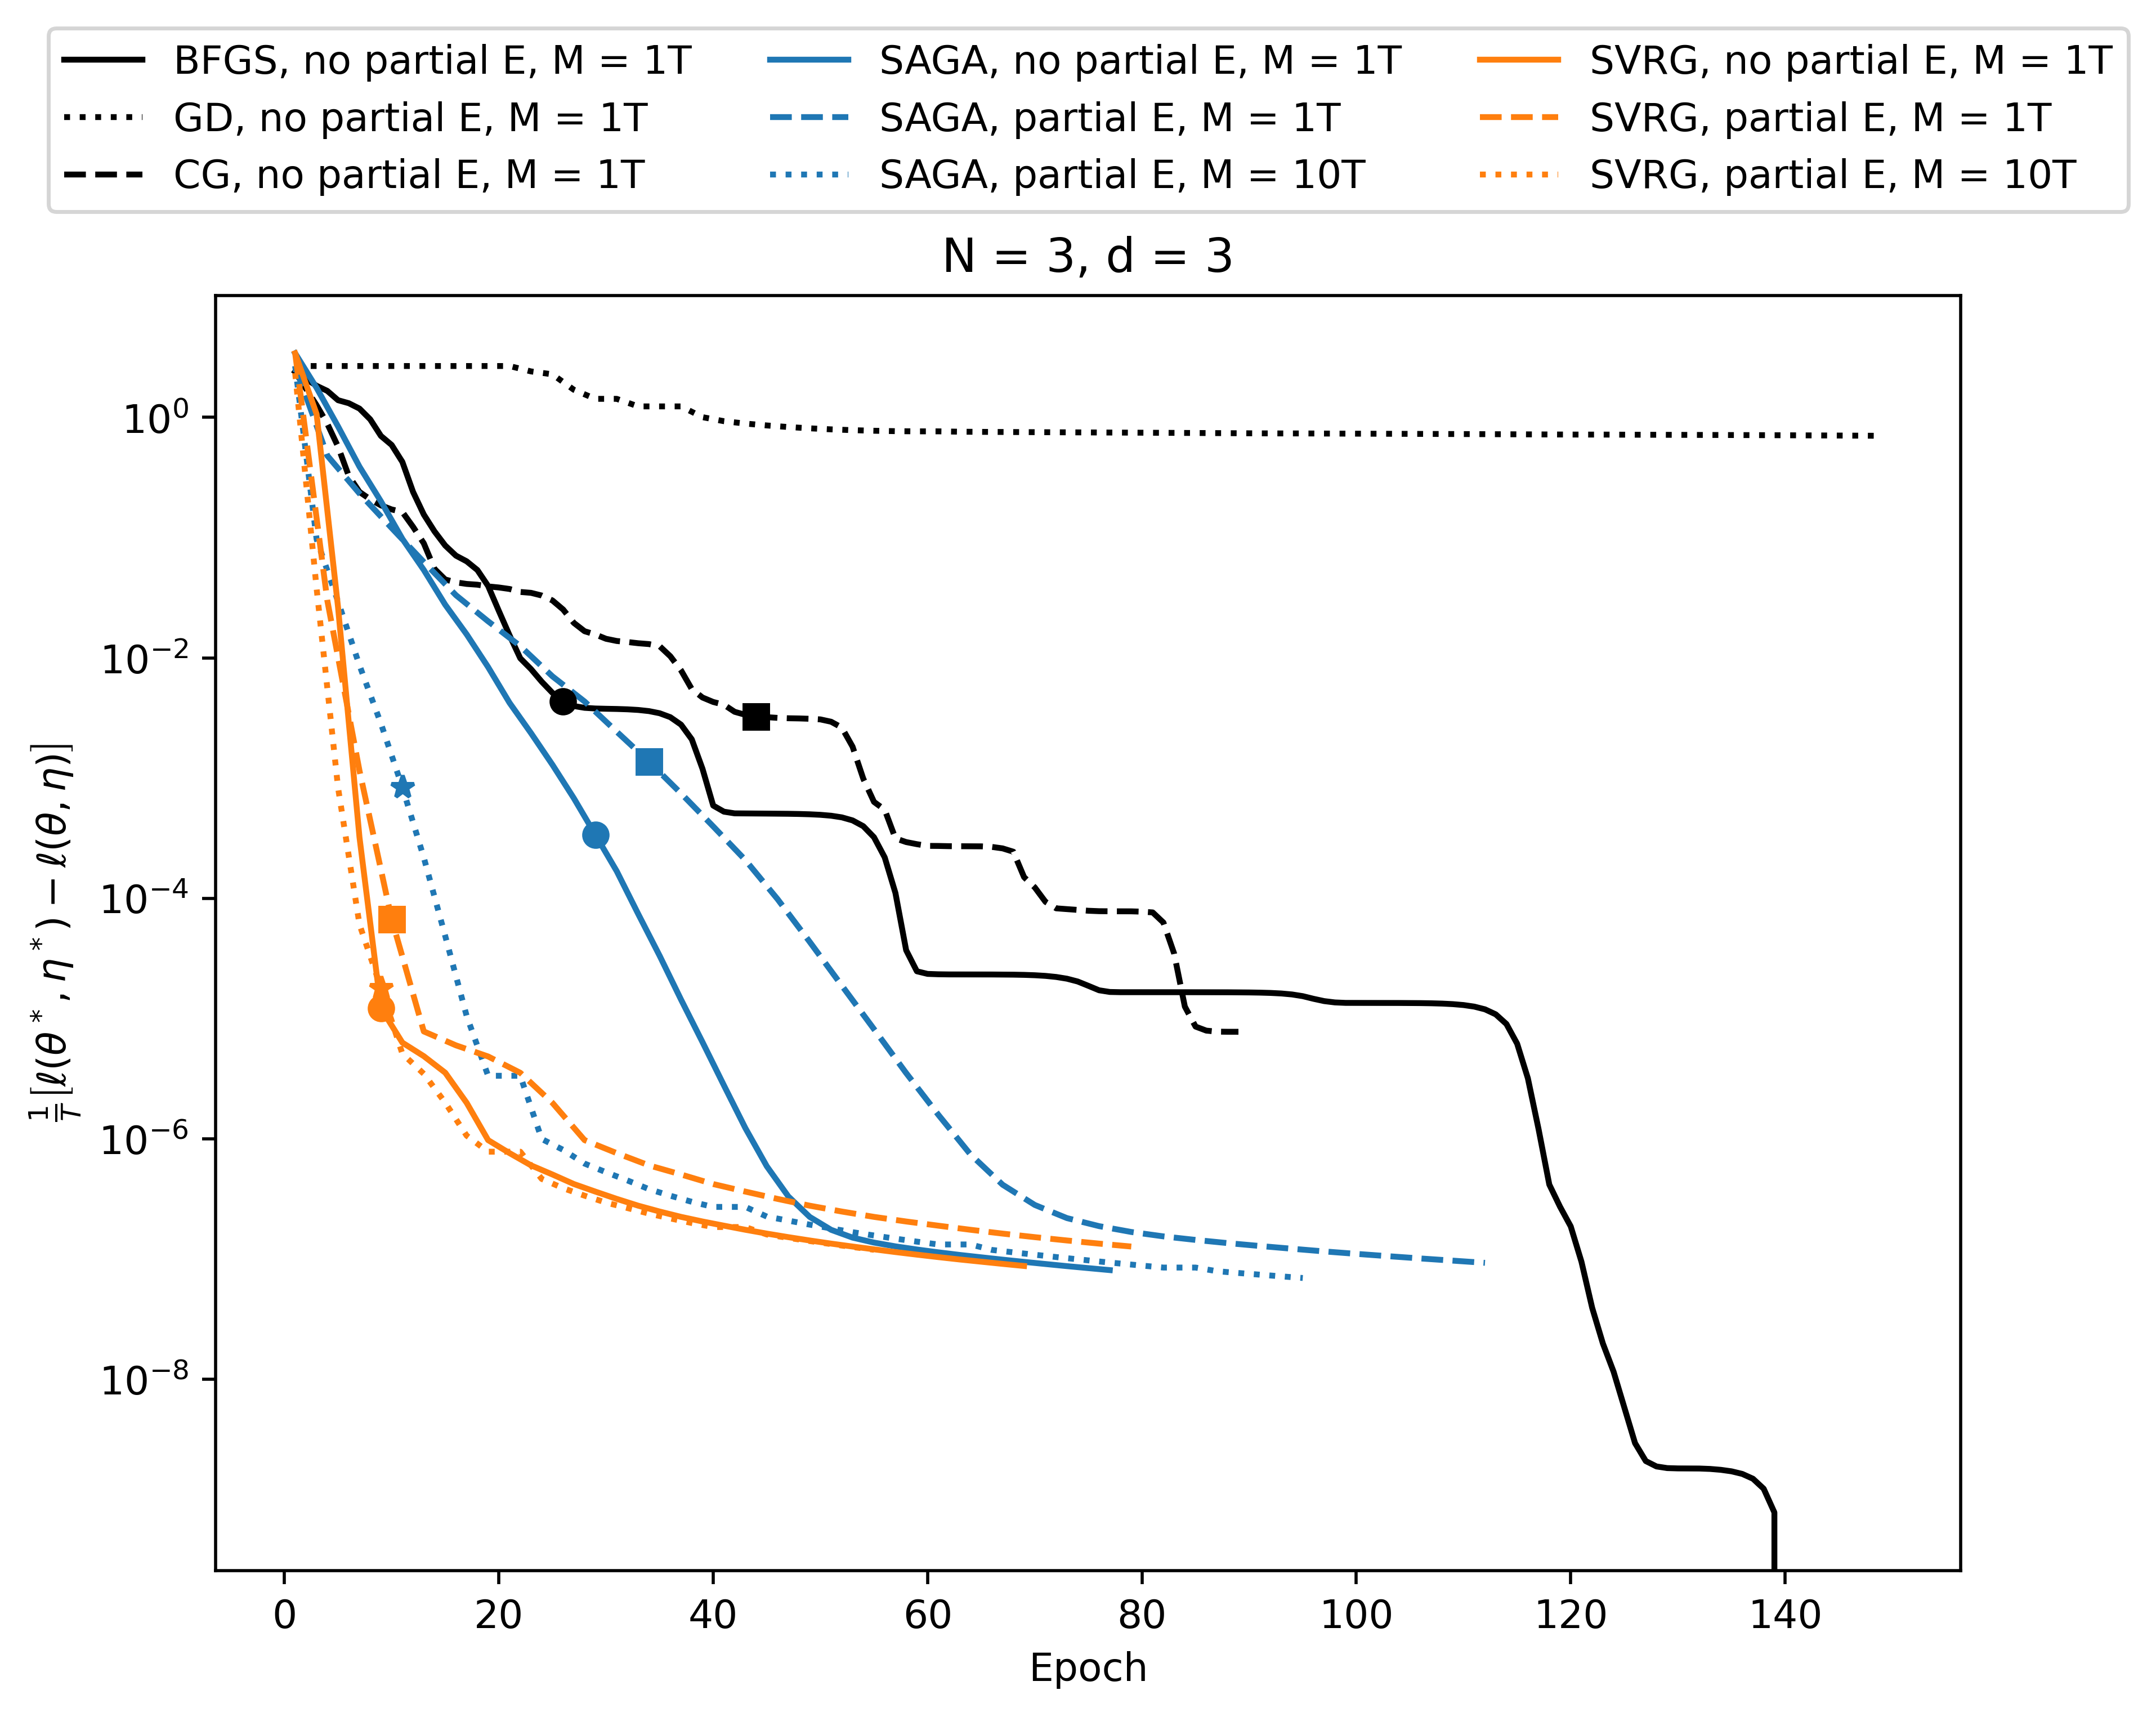
\includegraphics[width=3in]{../plt/log-like_v_epoch_T-100000-K-3-1-d-3-000.png}
    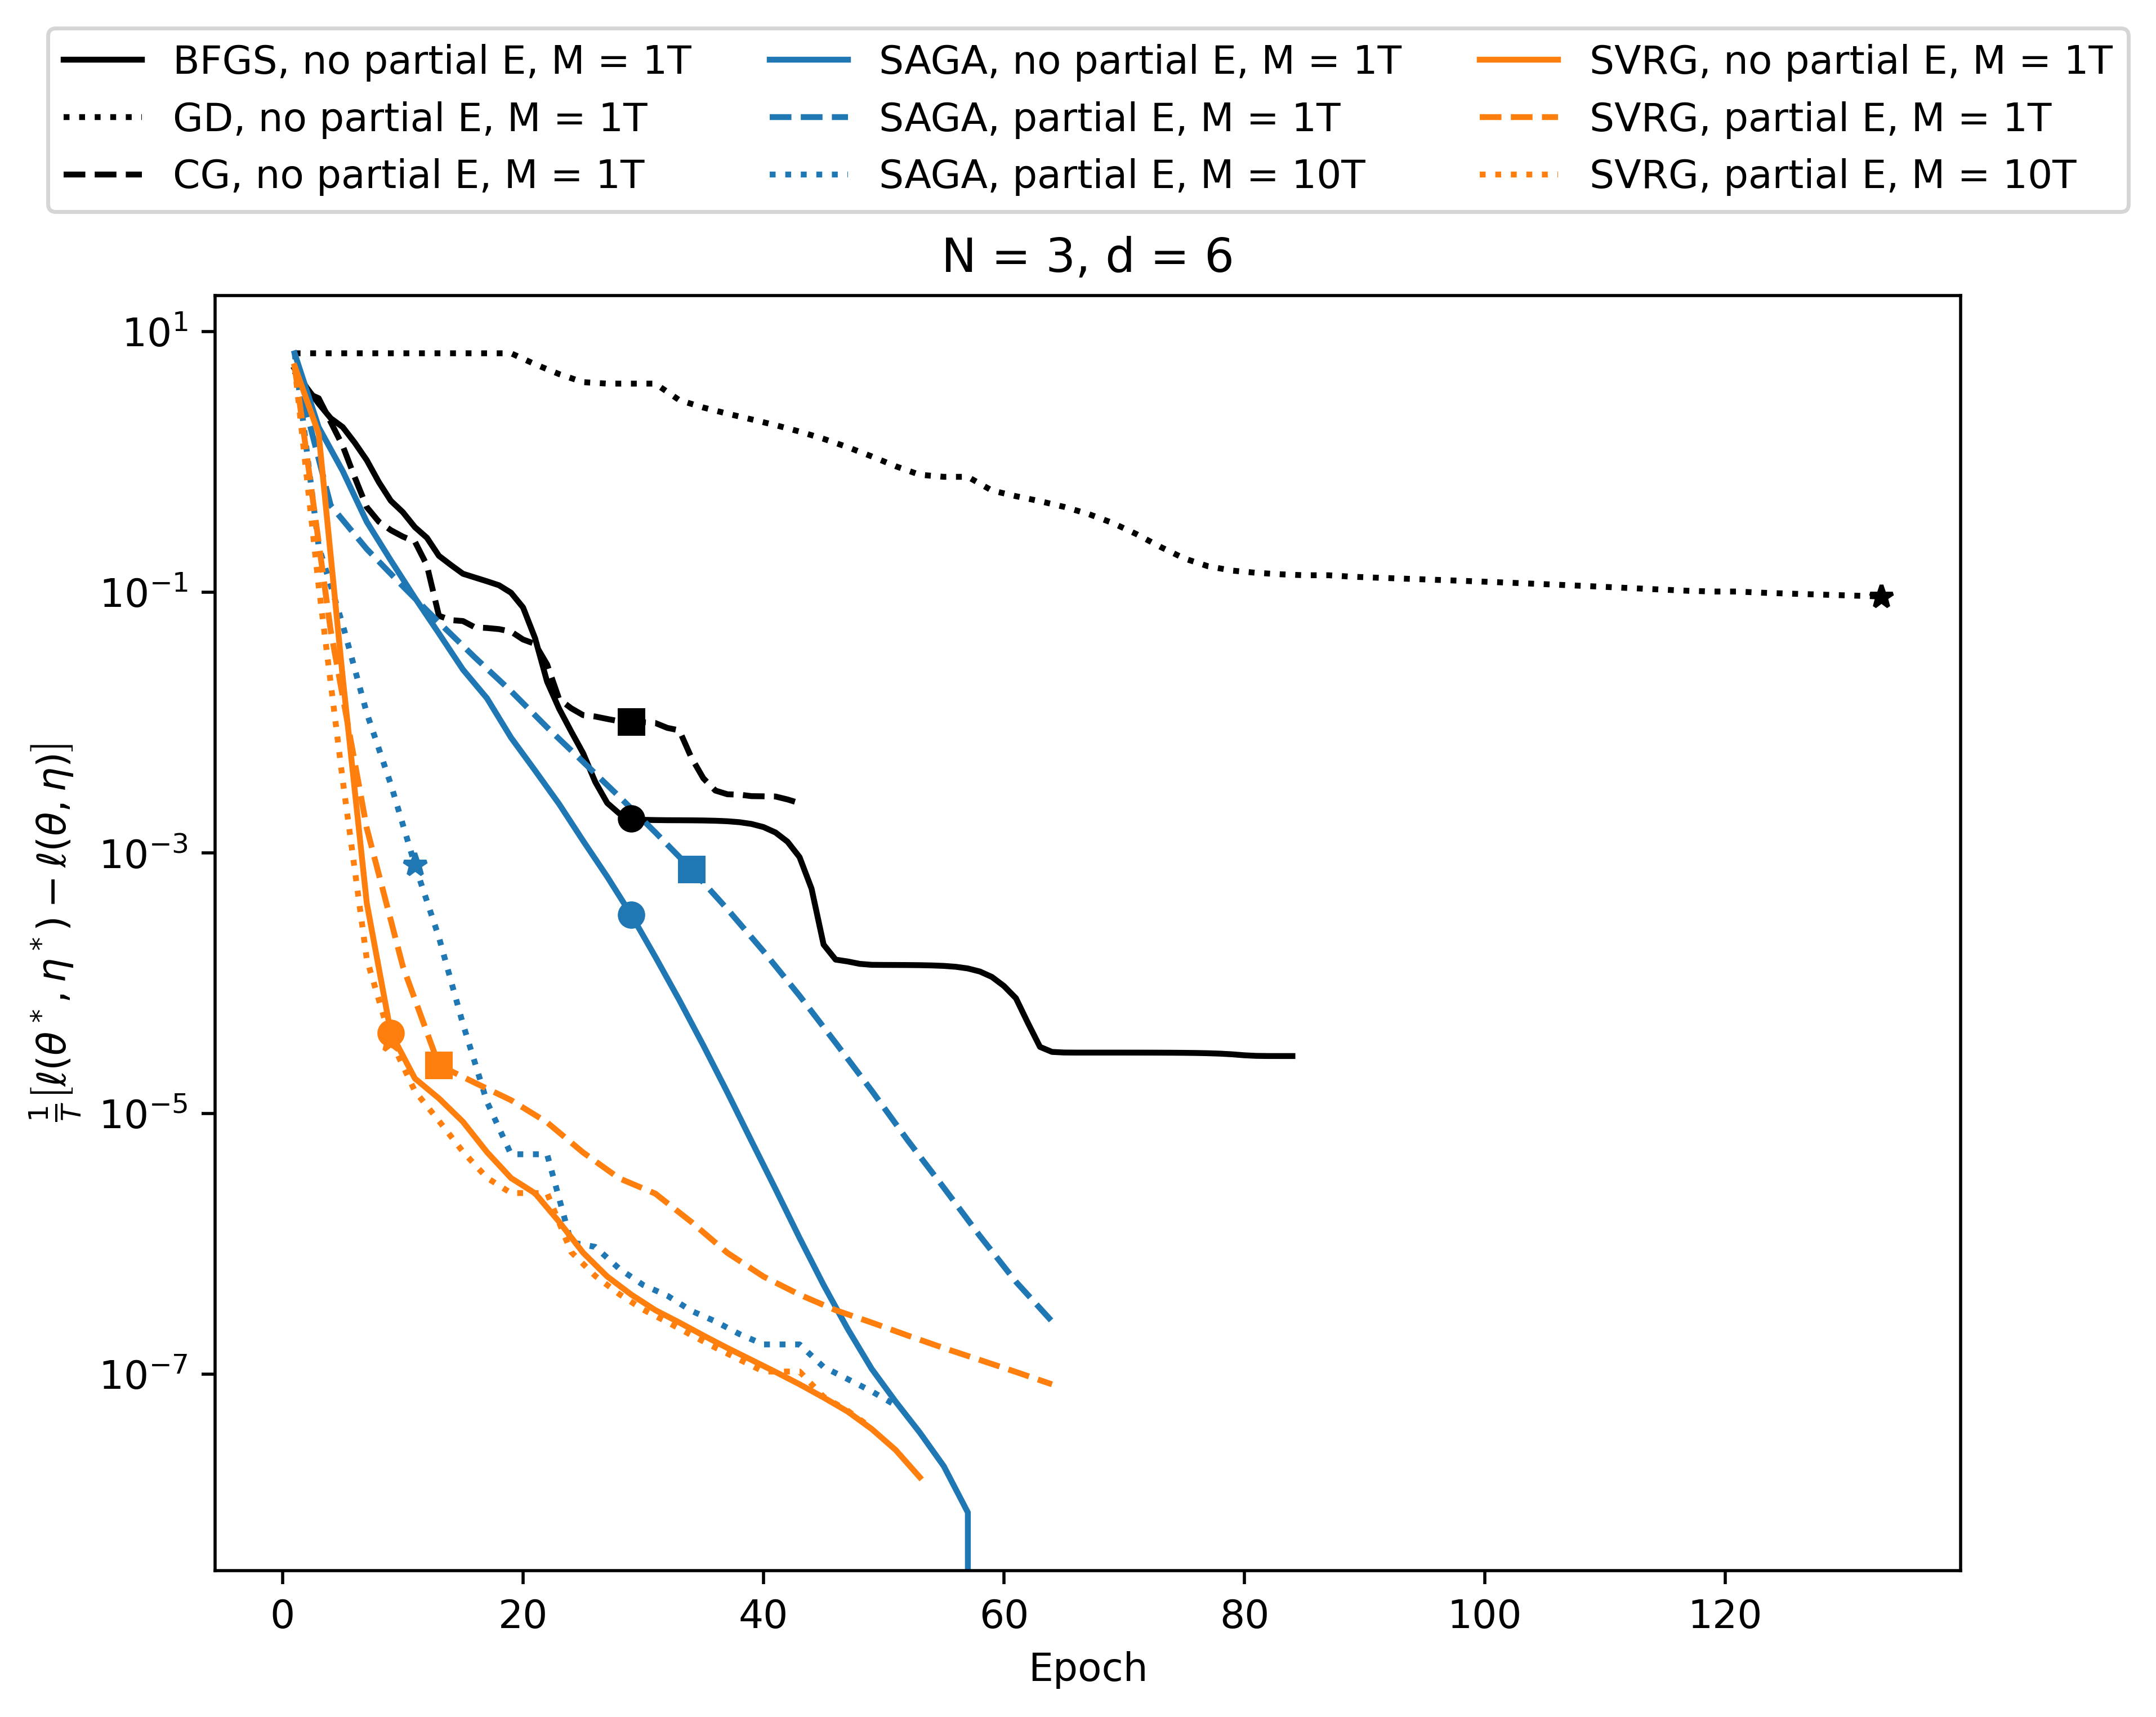
\includegraphics[width=3in]{../plt/log-like_v_epoch_T-100000-K-3-1-d-6-000.png}
    \\
    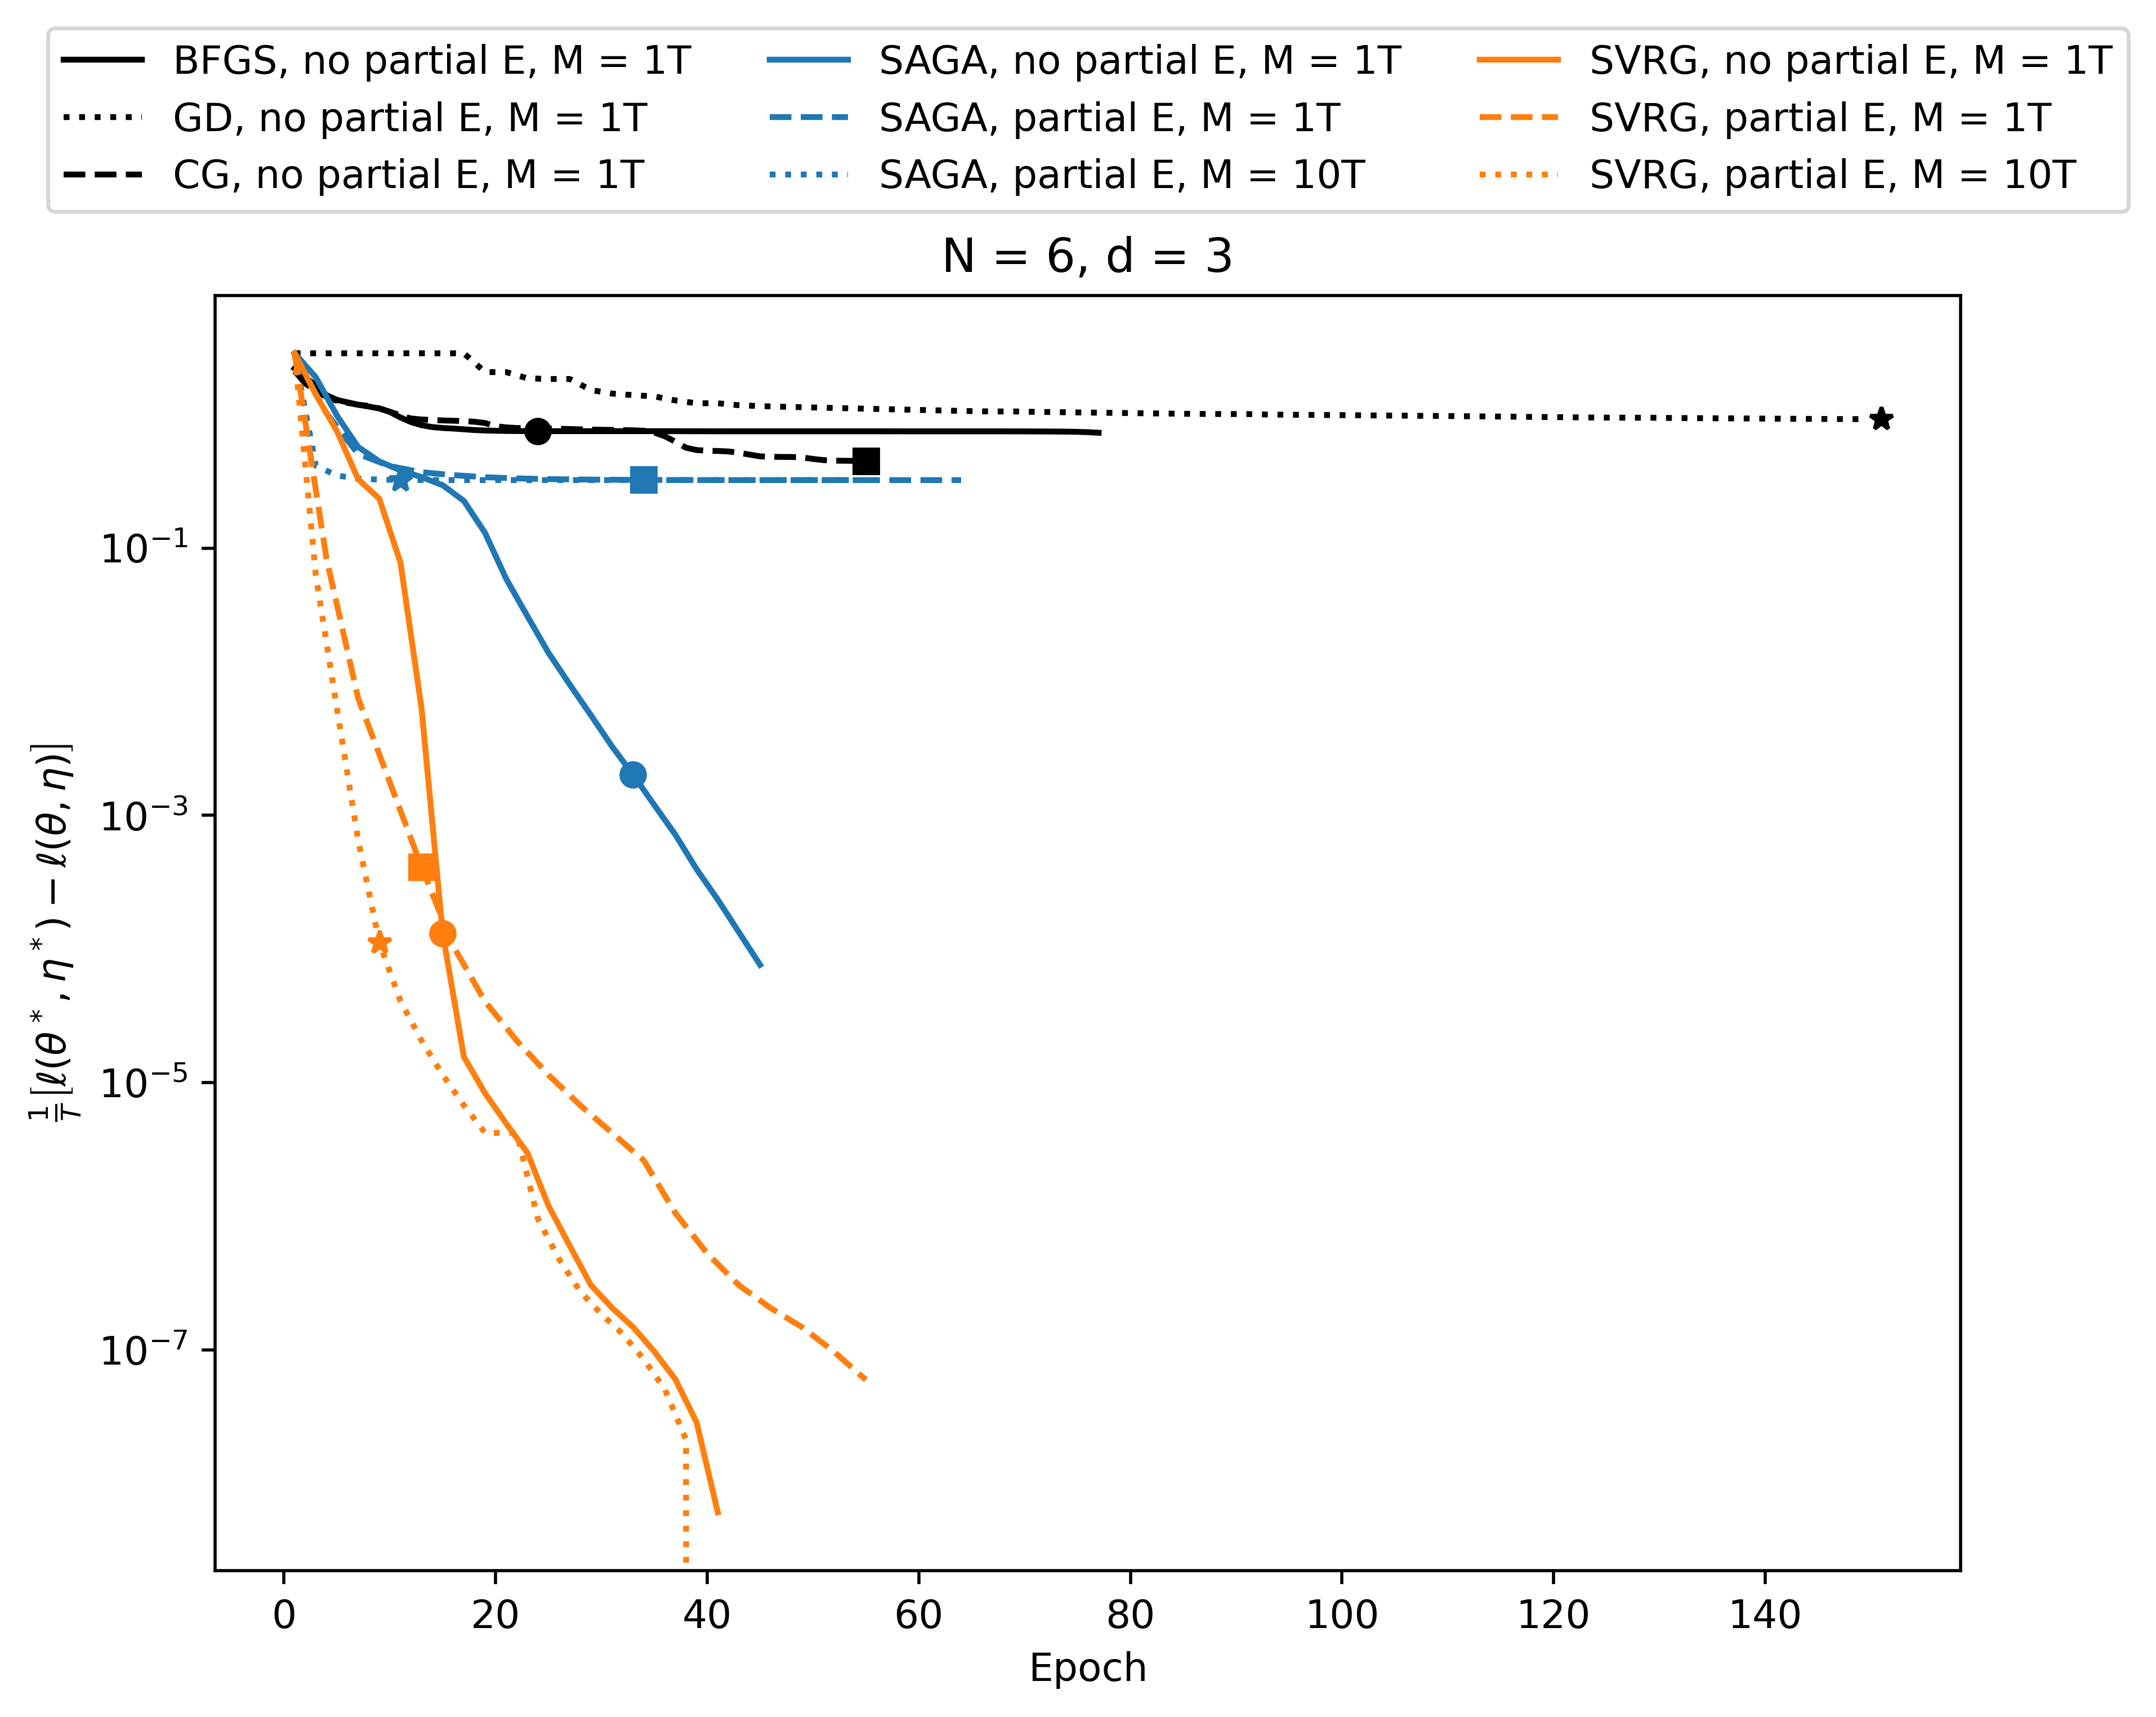
\includegraphics[width=3in]{../plt/log-like_v_epoch_T-100000-K-6-1-d-3-000.png}
    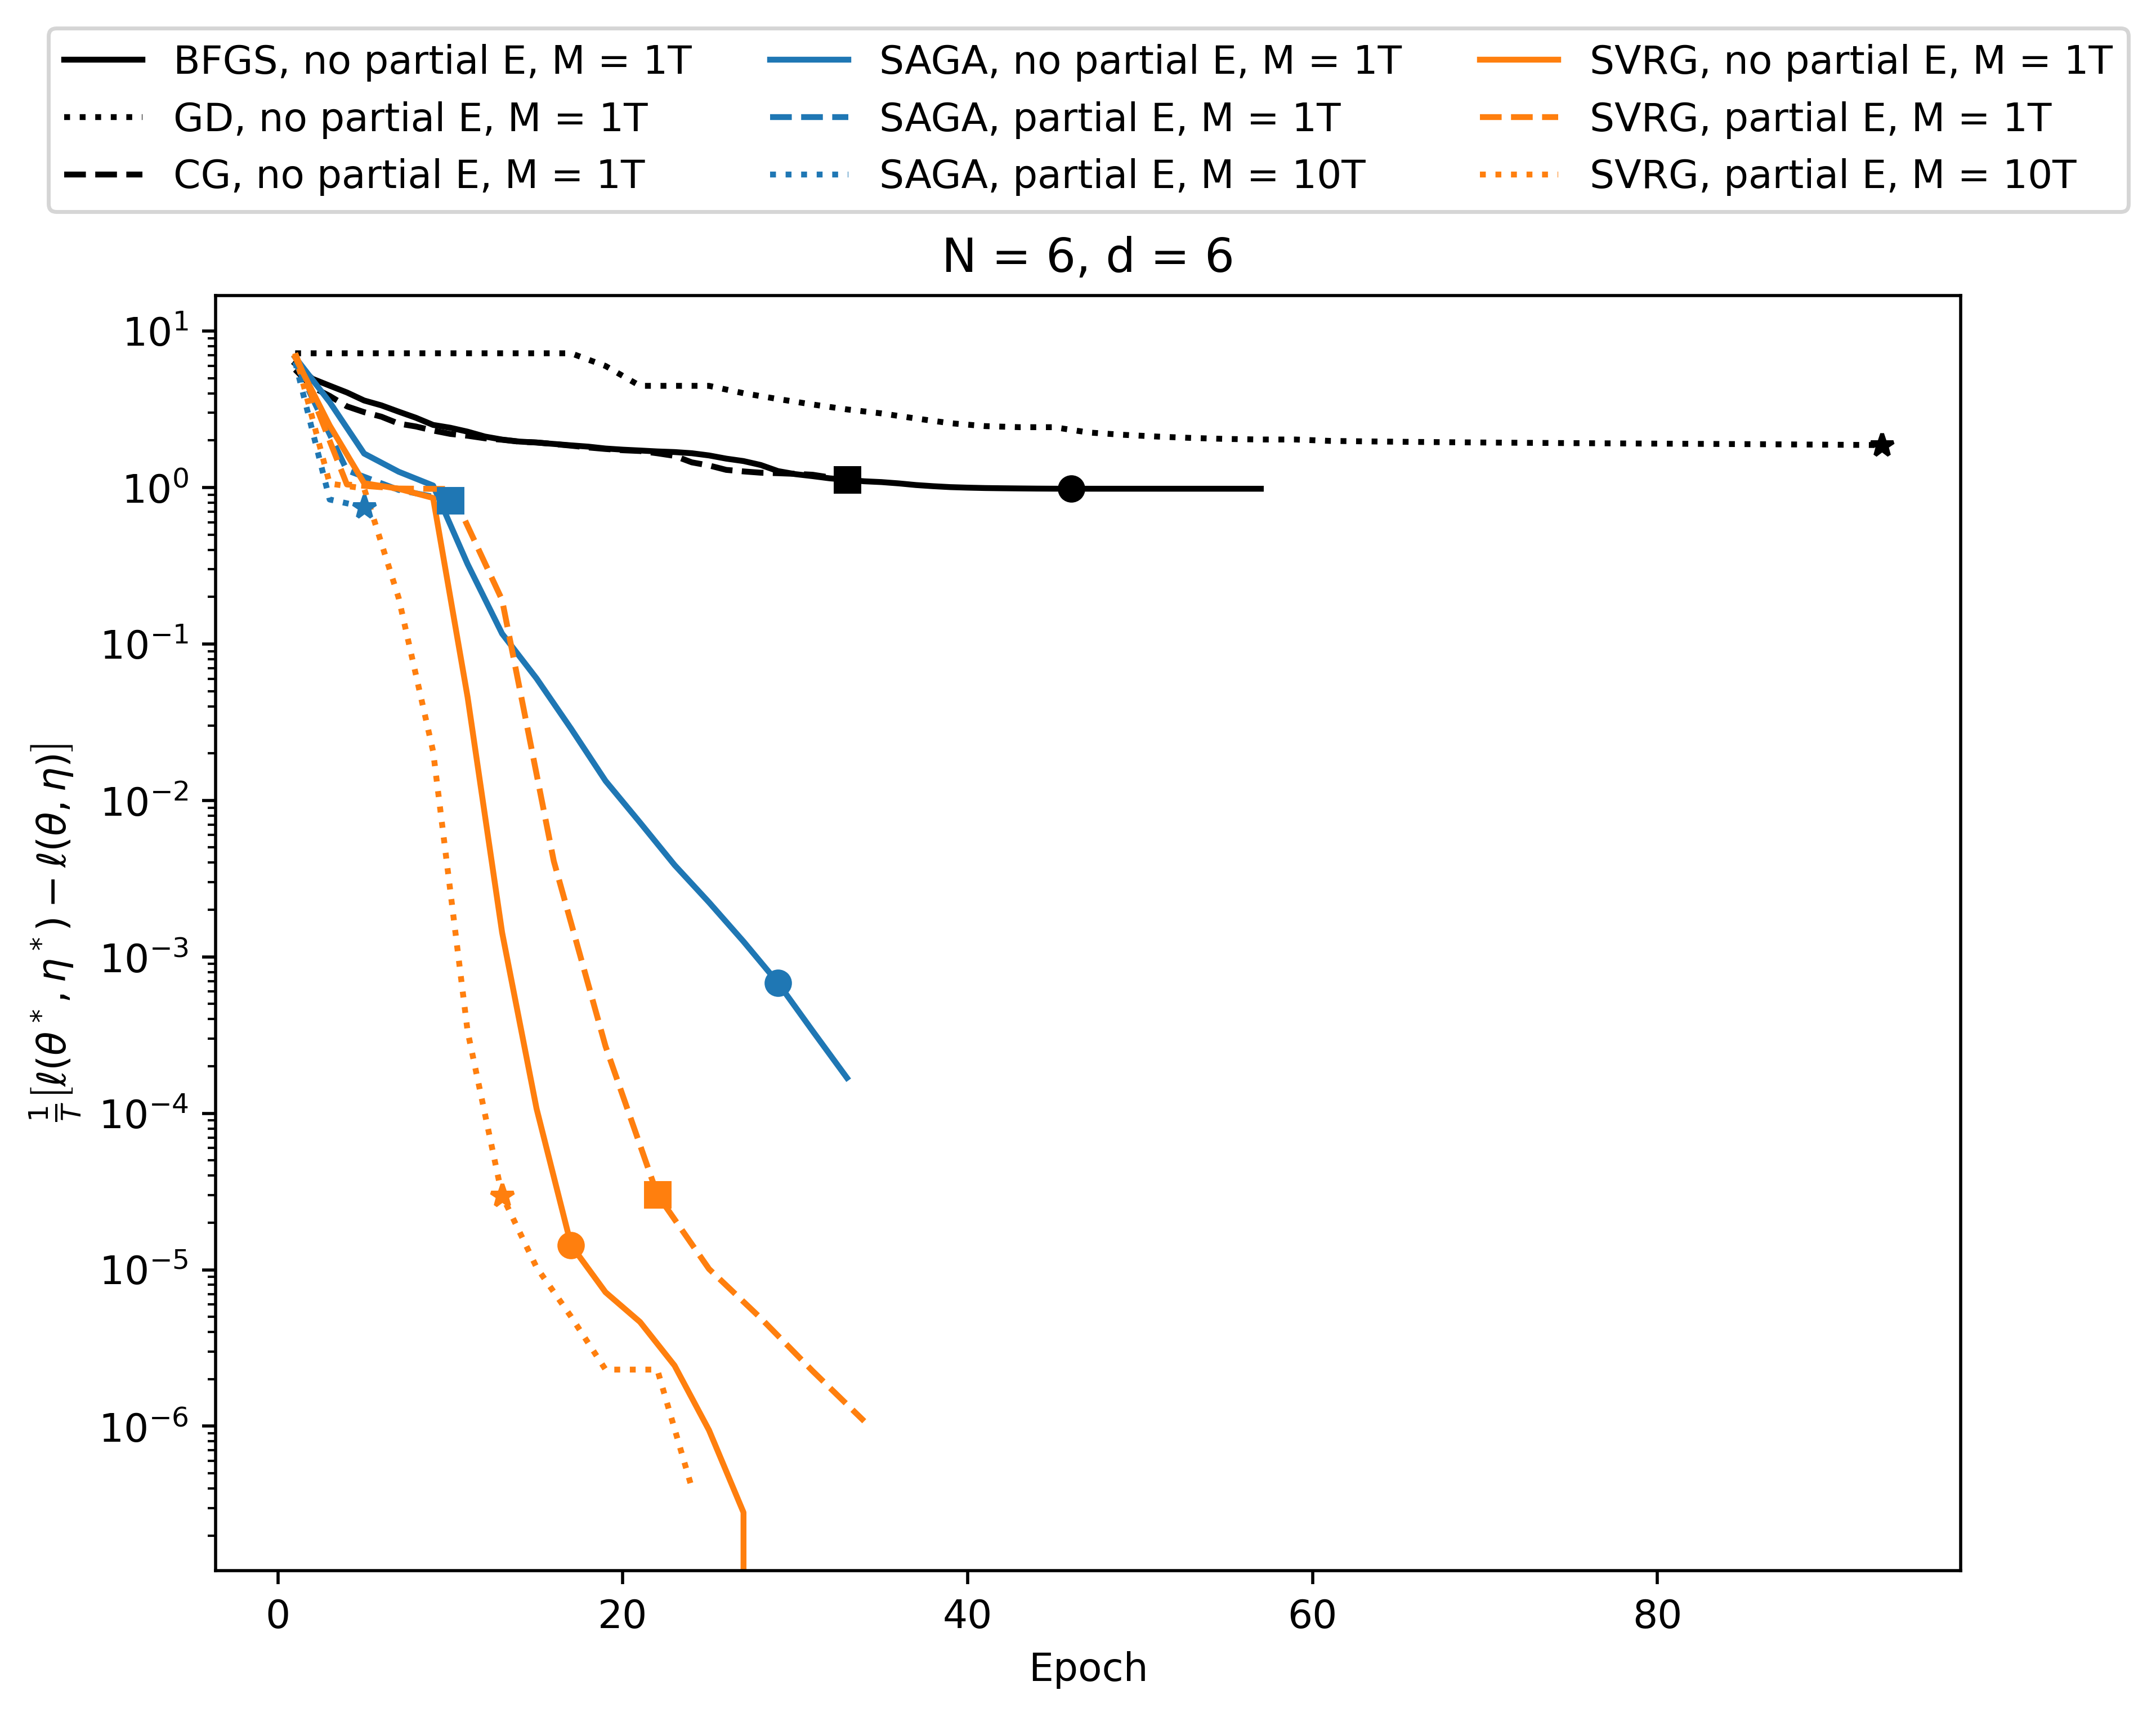
\includegraphics[width=3in]{../plt/log-like_v_epoch_T-100000-K-6-1-d-6-000.png}   
    \caption{Optimally gap between the log-likelihood and optimal log-likelihood for the estimated parameters of the HMM from simulation studies with $T=10^{5}$, $N=3$ and $d=3$ (top left), $N=3$ and $d=6$ (top right), $N=6$ and $d=3$ (bottom left), and $N=6$ and $d=6$ (bottom left). One epoch represents either one full E-step, $T$ iterations with the M-step, or one gradient step for full-gradient algorithms. The y-axis is on a log-scale.}
    \label{fig:ll_trace_sim}
\end{figure}
%
Figure (\ref{fig:boxplots_sim}) shows box plots of both the number of epochs until convergence as well as the optimality gap (log likelihood divided by $T$) at convergence for each algorithm. Convergence is defined as the point at which the gradient norm of the log-likelihood (divided by $T$) was less than $10^{-2}$. We selected a tolerance of $10^{-2}$ because it was the lowest tolerance that all algorithms regularly converged to within 12 hours. 
%
\begin{figure}
    \centering
    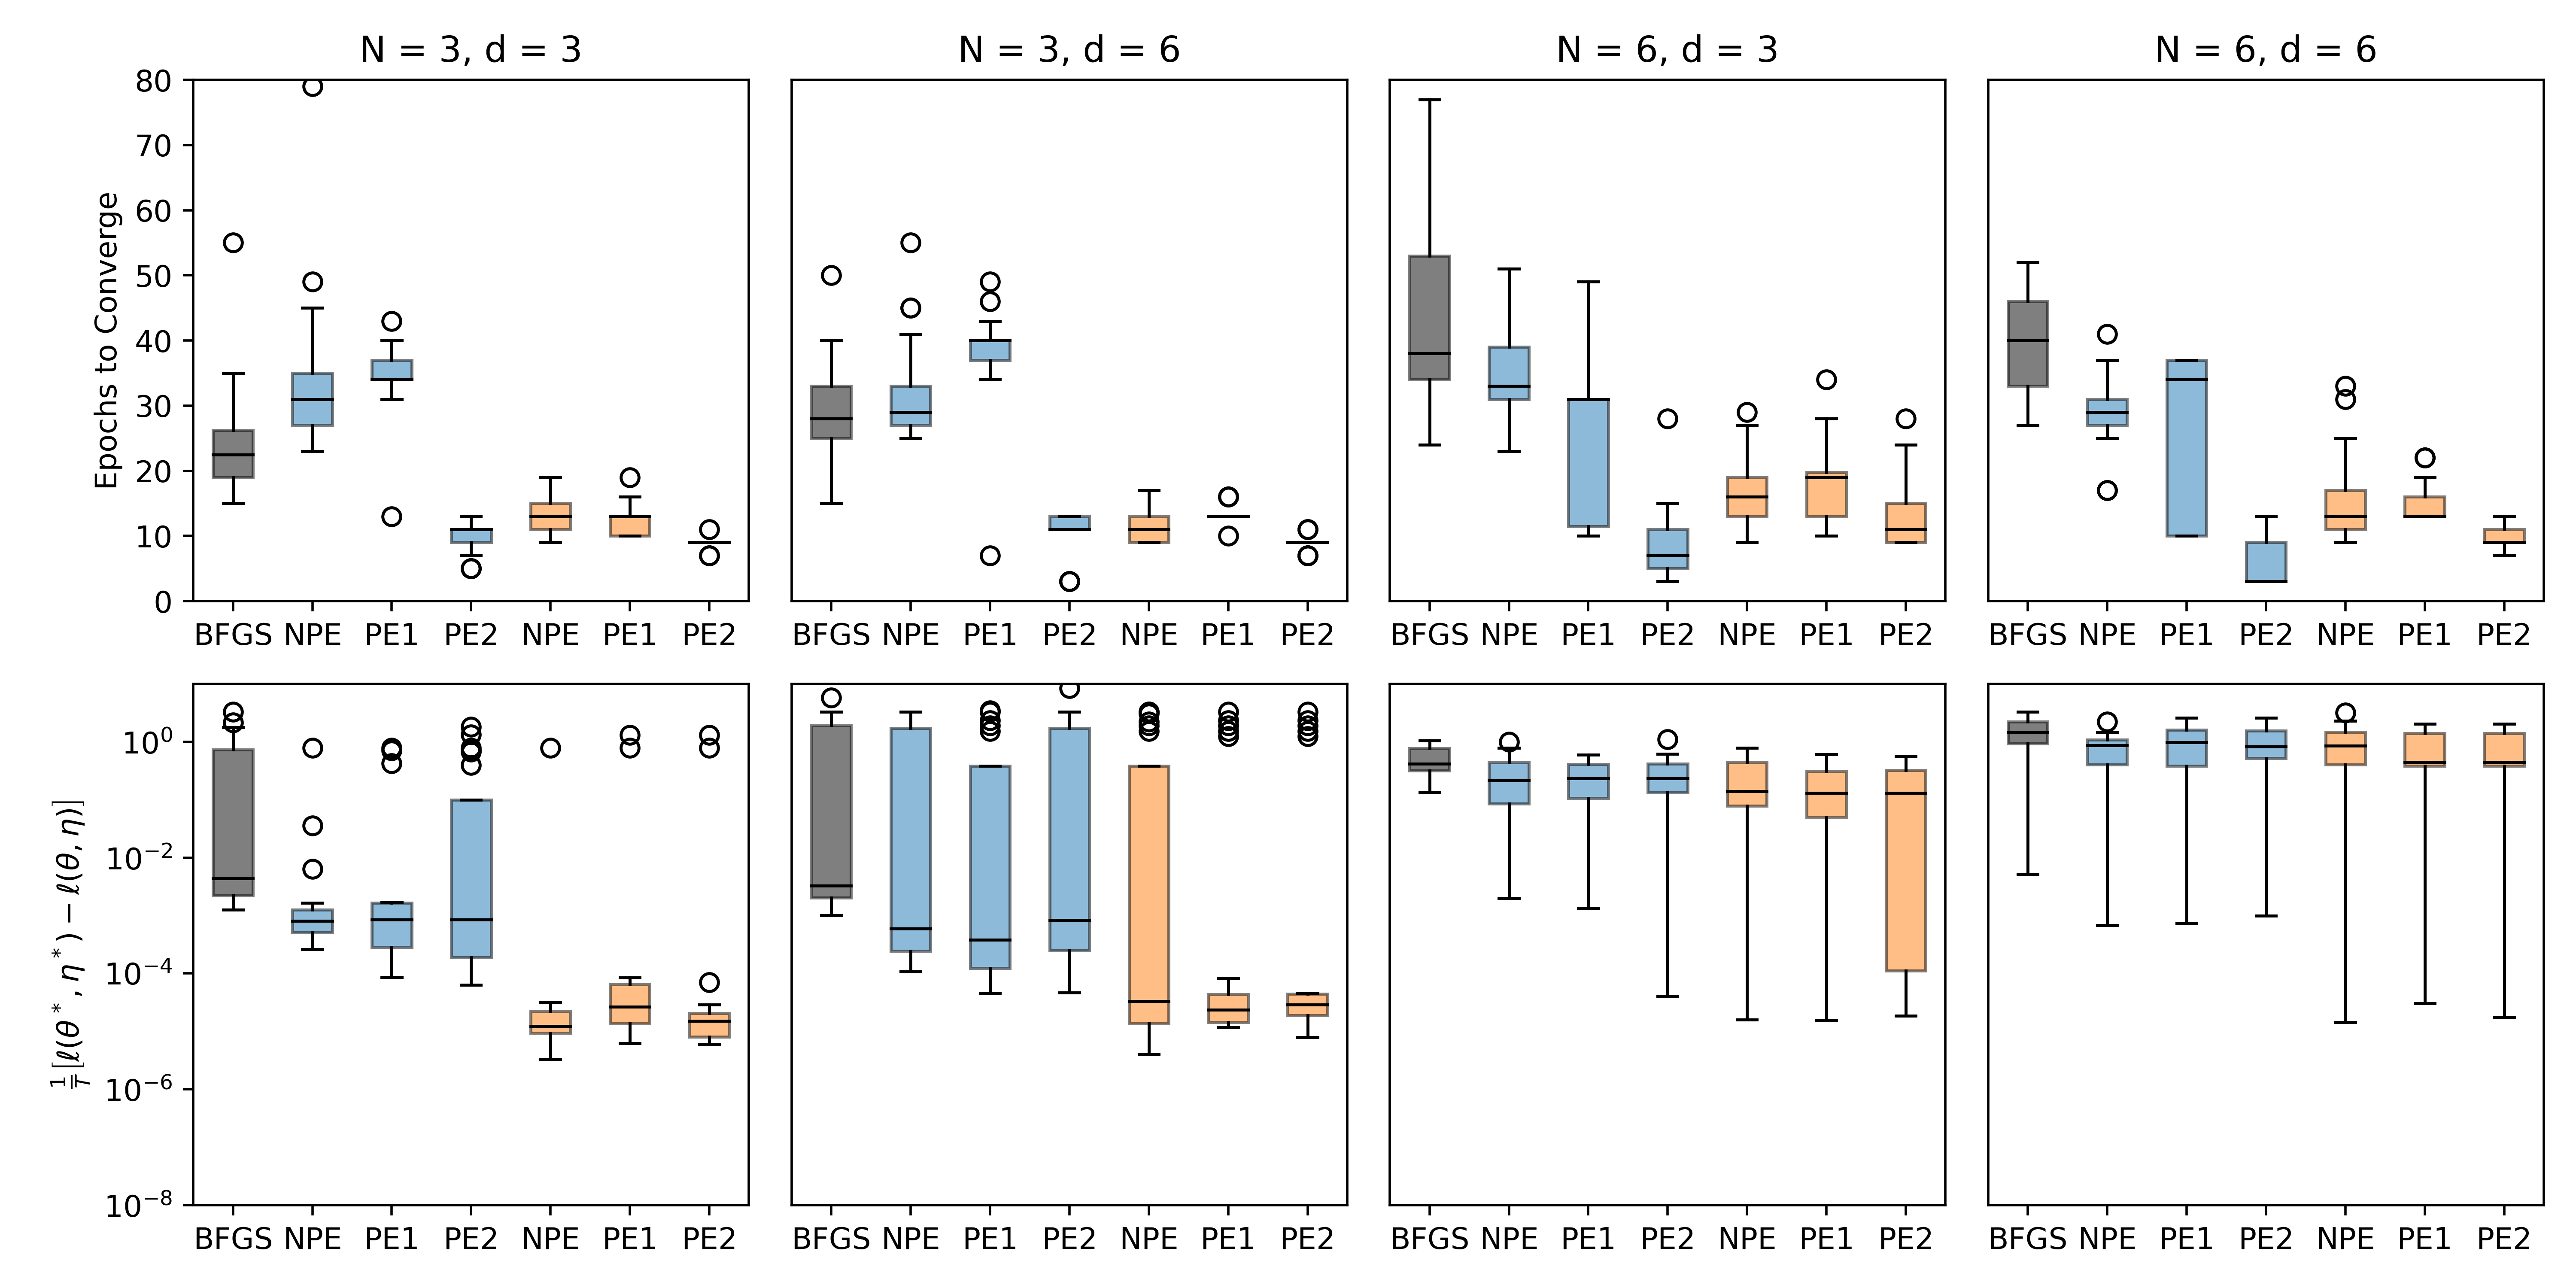
\includegraphics[width=6.5in]{../plt/boxplots_sim.png}
    \caption{Optimally gap between the log-likelihood and optimal log-likelihood for the estimated parameters of the HMM from simulation studies with $T=10^{5}$, $N=3$ and $d=3$ (top left), $N=3$ and $d=6$ (top right), $N=6$ and $d=3$ (bottom left), and $N=6$ and $d=6$ (bottom left). One epoch represents either one full E-step, $T$ iterations with the M-step, or one gradient step for full-gradient algorithms. The y-axis is on a log-scale.}
    \label{fig:scatter_sim}
\end{figure}
%
Figure (\ref{fig:scatterplots_sim}) displays scatter plots of the optimality gap vs the number of epochs until convergence.
%
\begin{figure}
    \centering
    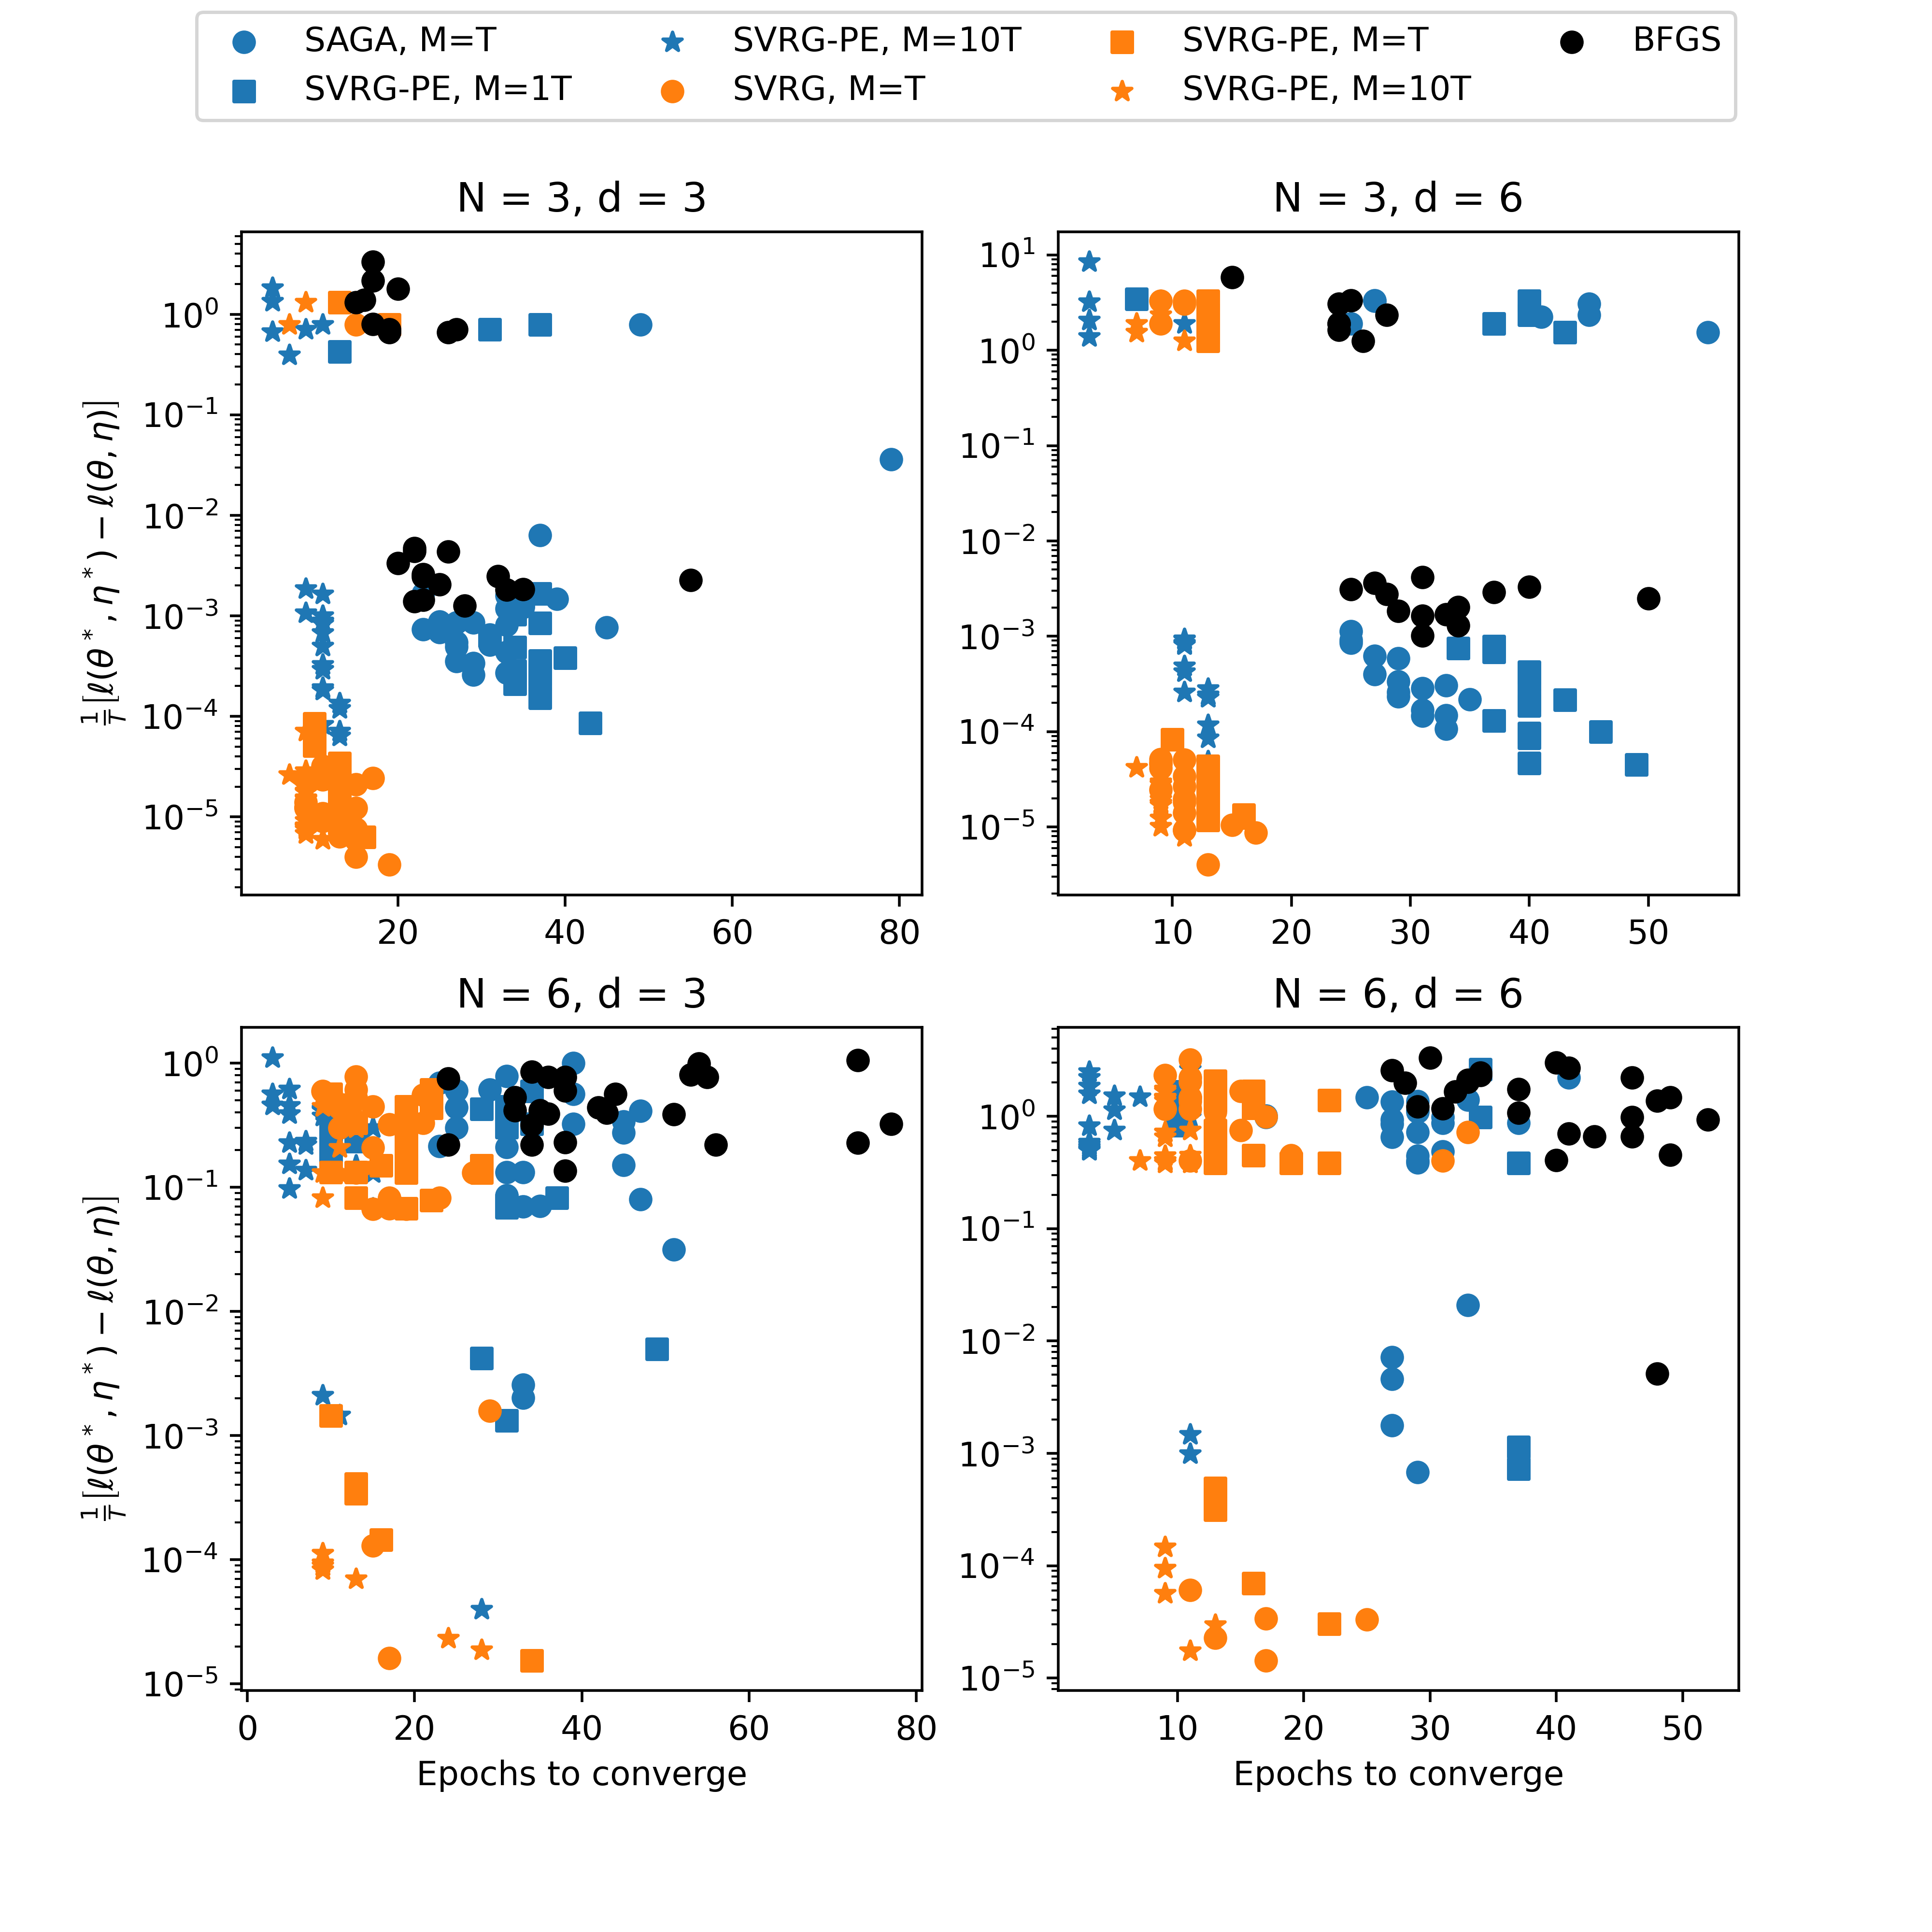
\includegraphics[width=6.5in]{../plt/scatter_sim.png}
    \caption{Optimally gap between the log-likelihood and optimal log-likelihood for the estimated parameters of the HMM from simulation studies with $T=10^{5}$, $N=3$ and $d=3$ (top left), $N=3$ and $d=6$ (top right), $N=6$ and $d=3$ (bottom left), and $N=6$ and $d=6$ (bottom left). One epoch represents either one full E-step, $T$ iterations with the M-step, or one gradient step for full-gradient algorithms. The y-axis is on a log-scale.}
    \label{fig:scatter_sim}
\end{figure}
%
Overall, SVRG appears to converge faster than SAGA for all algorithms. This may be a function of our step size ($1/3 \hat L$), but that step size was selected based upon suggestions from the SAGA paper \citep{Defazio:2014}. In addition SVRG converges faster than the baseline for all experiments, and SAGA converged faster than the baseline for all experiments except for perhaps when $N=3$. The baseline is prone to converging to local minima, especially when $N=6$. Our method still is prone to converge to local minima, especially when $N=6$, but it is performs better than BFGS for all experiments. IN particular, Figure (\ref{fig:scatter_sim}) shows than most SVRG / SAGA experiments converge faster and to solutions with higher likelihood compared to BFGS.

The partial E step looks to help primarily for experiments with $N=6$, especially for early epochs of the algorithm. This makes sense since the weights from the EM algorithm will be out of date quickly when the parameter estimates are poor early in the EM algorithm.

%SAGA without a partial E-step performs similarly to the EM algorithm in a per-epoch basis because SAGA is successfully converging for the M-step when $M = T$. However, it does not perform as well as the EM algorithm on a per-time basis because the M-step is significantly slower when using SAGA vs the closed-form solution. This behaviour is expected, and SAGA has a significant advantage over the EM algorithm in that it only requires gradients rather than sufficient statistics.

%mplementing a partial E-step shows that SAGA can outperform the EM algorithm when the parameter estimates are far from the optimal solutions and when the underlying HMM does not mix rapidly. This is likely because the weights of the $F$ and $G$ are very inaccurate at first, and updating them early in the optimization procedure yields a significant speed-up. In addition, if the Markov chain is rapidly mixing, then updates to $\gamma_{t_m}$ and $\xi_{t_m}$ at a single data point are more accurate. Future work may involve performing the partial-E step for many weights at once sequentially, depending upon the mixing time of the current estimate of $\eta_k$.